\newpage
МРНТИ 61.51.21

\sectionwithauthors{К.К.Сейлханов, Б.Т.Мурзагалиев, Ж.Т.Даулетжанова, М.Т.Сейлханова, С.Бахтияр}{МАТЕМАТИЧЕСКИЙ МЕТОД ОПРЕДЕЛЕНИЯ ТОВАРНОЙ ПРОДУКЦИИ ПРИ
ПЕРЕРАБОТКЕ И ПОДГОТОВКИ УГЛЕВОДОРОДНЫХ ГАЗОВ}

\begin{center}
{\bfseries \textsuperscript{1}К.К.Сейлханов,
\textsuperscript{1}Б.Т.Мурзагалиев,
\textsuperscript{2}Ж.Т.Даулетжанова\textsuperscript{🖂}, \textsuperscript{1}М.Т.Сейлханова, \textsuperscript{1}С.Бахтияр}

\textsuperscript{1}Товарищество с ограниченной ответственностью «ГЦПК
«Кəсіпкер», Астана, Казахстан,

\textsuperscript{2}Казахский университет технологии и бизнеса имени К.
Кулажанова, Астана, Казахстан

{\bfseries \textsuperscript{🖂}}Корреспондент-автор: Kaliyeva\_zhanna
@mail.ru
\end{center}

В научной статье описан математический метод расчета количеств
углеводородных газов на разных этапах переработки углеводородного сырья,
начиная от смешивания потоков углеводородного сырья и заканчивая
контролем точности выходов продукции. Такой комплексный подход
обеспечивает системное улучшение всех процессов переработки. Научная
статья содержит примеры расчетов, что делает методику доступной для
использования специалистами в отрасли. Это позволяет легко адаптировать
и применять предложенные методы в различных производственных условиях.
Эти аспекты подчеркивают высокую значимость и инновационность
выполненной научной работы, способствуя решению актуальных проблем
переработки углеводородного сырья и повышению эффективности
нефтехимической промышленности.

{\bfseries Ключевые слова:} углеводородные газы, состав газа, методика
расчета газовых смесей, материальный баланс газовых смесей.

\sectionheading{КӨМІРСУТЕК ГАЗДАРЫН ӨҢДЕУ ЖӘНЕ ДАЙЫНДАУ КЕЗІНДЕ ТАУАРЛЫҚ
ӨНІМДЕРДІ АНЫҚТАУДЫҢ МАТЕМАТИКАЛЫҚ ӘДІСІ}

\begin{center}
{\bfseries \textsuperscript{1}К.К.Сейлханов,
\textsuperscript{1}Б.Т.Мурзагалиев,
\textsuperscript{2}Ж.Т.Даулетжанова\textsuperscript{🖂},}

{\bfseries \textsuperscript{1}М.Т.Сейлханова, \textsuperscript{1}С.Бахтияр}

\textsuperscript{1}Жауапкершілігі шектеулі серіктестік «ГЦПК «Кəсіпкер»,
Астана, Қазақстан

\textsuperscript{2}Қ.Құлажанов атындағы Қазақ технология және бизнес
университеті, Астана, Қазақстан,

e-mail: Kaliyeva\_zhanna @mail.ru
\end{center}

Ғылыми мақалада көмірсутектерді өңдеудің әртүрлі кезеңдерінде
көмірсутекті қоректік ағындарды араластырудан бастап өнім шығымының
дәлдігін бақылауға дейін көмірсутекті газдардың мөлшерін есептеудің
математикалық әдісі сипатталған. Бұл кешенді тәсіл өңдеудің барлық
процестерін жүйелі түрде жақсартуды қамтамасыз етеді. Ғылыми мақалада
есептеу мысалдары келтірілген, бұл әдістемені сала мамандарына
қолжетімді етеді. Бұл ұсынылған әдістерді әртүрлі өндірістік жағдайларда
бейімдеуді және қолдануды жеңілдетеді.Бұл аспектілер көмірсутегін
өңдеудің өзекті мәселелерін шешуге және мұнай-химия өнеркәсібінің
тиімділігін арттыруға ықпал ететін атқарылған ғылыми жұмыстардың жоғары
маңыздылығы мен жаңашылдығын көрсетеді.

{\bfseries Түйін сөздер:} көмірсутекті газдар, газ құрамы, газ қоспаларын
есептеу әдістері, газ қоспаларының материалдық балансы.

\sectionheading{MATHEMATICAL METHOD FOR DETERMINING COMMERCIAL PRODUCTS DURING
PROCESSING AND PREPARATION OF HYDROCARBON GASES}

\begin{center}
{\bfseries \textsuperscript{1}K.K.Seilkhanov,
\textsuperscript{1}B.T.Murzagaliev, \textsuperscript{2}Zh.T.
Dauletzhanova\textsuperscript{🖂},}

{\bfseries \textsuperscript{1}M.T.Seilkhanova,
\textsuperscript{1}S.Bakhtiyar}

\textsuperscript{1}Limited liability partnership «ГЦПК «Кəсіпкер»,
Astana, Kazakhstan,

\textsuperscript{2}Kazakh University of Technology and Business named
after K. Kulazhanov, Astana, Kazakhstan,

e-mail: Kaliyeva\_zhanna @mail.ru
\end{center}

The scientific article describes a mathematical method for calculating
the amounts of hydrocarbon gases at different stages of hydrocarbon
processing, starting from mixing hydrocarbon feed streams and ending
with monitoring the accuracy of product yields. This integrated approach
ensures systemic improvement of all processing processes. The scientific
article contains examples of calculations, which makes the methodology
accessible for use by industry specialists. This makes it easy to adapt
and apply the proposed methods in various production conditions. These
aspects emphasize the high significance and innovativeness of the
scientific work performed, contributing to solving pressing problems of
hydrocarbon processing and increasing the efficiency of the
petrochemical industry.

{\bfseries Key words:} hydrocarbon gases, gas composition, methods for
calculating gas mixtures, material balance of gas mixtures.

\begin{multicols}{2}
{\bfseries Введение.} В последние годы все большую долю сырья в
нефтехимической промышленности занимают попутные газы нефтяных
месторождений. Добыча, транспортировка, переработка и хранение
углеводородного сырья, такого как природный газ и попутный нефтяной газ,
играет ключевую роль в нефтехимической промышленности и энергетическом
секторе {[}1{]}. Повышение эффективности переработки углеводородного
сырья может значительно повысить экономическую эффективность
нефтегазовых компаний и улучшить экономические показатели страны.
Интеграция современных технологий - внедрение современных методов
вычислений технологии разделения, адсорбционные и абсорбционные
процессы, позволяет значительно улучшить процесс переработки
углеводородного сырья и повысить выход целевых продуктов {[}2{]}.

Сокращение выбросов загрязняющих веществ и парниковых газов является
приоритетом в глобальной экологии. Эффективная переработка попутного
нефтяного газа позволяет уменьшить объемы сжигания газа на факелах, что
способствует снижению экологической нагрузки на окружающую среду
{[}3{]}.

Переработка углеводородного сырья, такого как природный газ, попутный
нефтяной газ или иной углеводородный газ, является актуальным, сложным
многоэтапным процессом. На каждом этапе переработки происходит выделение
различных продуктов, включая товарный газ, сжиженный нефтяной газ,
сжиженный углеводородный газ, конденсат и другие углеводороды. Для
обеспечения точности в определении количества этих продуктов
используются различные методики, основанные на материальных балансах,
физических и химических свойствах сырья, а также на данных, полученных с
помощью аналитических методов {[}4{]}.

Определение количества товарного газа, СНГ, СУГ, конденсата и других
продуктов при переработке углеводородного сырья является критически
важным этапом, влияющим на экономическую эффективность и экологическую
безопасность производства. Развитие методов материального баланса,
использование передовых аналитических технологий и оптимизация
технологических процессов позволяют достигать высокой точности и
надежности расчетов. Важное значение имеет также постоянное
совершенствование технологических установок и внедрение инновационных
решений, направленных на снижение потерь и минимизацию воздействия на
окружающую среду {[}5{]}.

Месторождения углеводородного сырья часто расположены в отдаленных
районах, что делает транспортировку газа капиталоемкой. Разработка
методов переработки газа непосредственно на месте его добычи может
существенно снизить затраты на транспортировку и повысить рентабельность
производства. Методы расчета количества углеводородной продукции играют
ключевую роль в повышении экономической и экологической эффективности
процессов переработки углеводородного сырья. Точные расчеты материальных
балансов и использование передовых аналитических технологий позволяют
оптимизировать производственные процессы, снизить затраты и уменьшить
негативное воздействие на окружающую среду. Применение этих методов
способствует достижению устойчивого развития нефтегазовой
промышленности, обеспечивая баланс между экономическими выгодами и
экологической ответственностью.

Проекты по сокращению объемов сжигания ПНГ носят, в основном,
экологическую направленность. Положительный эффект заключается в
снижении выбросов значительного количества загрязняющих веществ (ЗВ) и
парниковых газов в атмосферу. Исторически нормативно-правовые акты и
регулирующие документы в России недостаточно стимулировали нефтяные
компании к минимизации факельного сжигания газа и повышения уровня его
эффективного использования {[}6{]}.

{\bfseries Материалы и методы.} В настоящее время использование механизмов
Киотского протокола помогают за счет продажи единиц сокращения выбросов
(ЕСВ) снизить уровень антропогенного воздействия на окружающую среду, а
также значительно улучшить экономические показатели проектов
эффективного использования ПНГ и компенсировать часть затрат на создание
инфраструктуры для утилизации попутного газа {[}7{]}. В настоящее время
вследствие ужесточения требований по выбросам ЗВ возникли
соответствующие нормативы, по которым в факелах разрешается сжигать не
более 5 \% произведенного ПНГ. При повышении этого уровня к плате за
выбросы ЗВ дополнительно применяются повышающие коэффициенты. Если узлы
учета ПНГ не установлены, данный коэффициент применяется равным 120.
Штрафы за сжигание ПНГ относительно невысоки, но снижение цены на нефть
и так привело к достаточно большим убыткам для нефтяных компаний
{[}8{]}. Во многих странах проекты добычи трудноизвлекаемой нефти
вследствие снижения цен стали нерентабельными. В России уже
приостановлены разработки некоторых новых нефтяных месторождений.
Поскольку для нефтехимической промышленности ПНГ является основным
сырьем, без которого она не может функционировать, длительная
эксплуатация существующих месторождений, без ввода новых, может привести
к дефициту сырья для нефтегазохимической промышленности, которая на
сегодняшний день, в среднем, загружена всего лишь на 40 \%. Учитывая то,
что на долю нефтехимической промышленности приходится около 60\%
промышленной продукции страны и более 7\% налоговых платежей, допущение
такой ситуации сильно отразится на экономике страны.

Низкий уровень утилизации ресурсов нефтехимии является одной из наиболее
острых современных проблем в развитии нефтегазового сектора России
{[}9{]}.

Подробная схема приведена на рис.1. пластовая газожидкостная смесь
поступает в блоки пробкоуловителей \emph{1}, где происходит разделение
газожидкостной смеси на газ углеводородный и конденсат. От блоков
пробкоуловителя \emph{1} газ направляется через аппарат воздушного
охлаждения \emph{3} на установку адсорбционной осушки, в состав которой
входят фильтры-сепараторы \emph{7} и группа адсорберов \emph{8}. По мере
заполнения адсорбционного слоя влагой, каждый из адсорберов выводится в
режим «регенерации» горячим газом, после чего охлаждается и включается в
режим «осушки». Осушенный газ от установки адсорбционной осушки двумя
параллельными потоками подается в блоки теплообменников. Первый поток:
блок теплообменников \emph{9}, где охлаждается до температуры минус
5--15°С газом из низкотемпературного сепаратора \emph{13}. Второй поток:
блок теплообменников \emph{10}, где охлаждается до температуры минус
25--35°С газовым конденсатом из низкотемпературного сепаратора \emph{13}
. Смешанный газ от теплообменников \emph{9}, \emph{10} с температурой
минус 20--30°С подается в промежуточные сепараторы \emph{11}, а затем на
турбодетандерного агрегата \emph{12}, где температура газа понижается до
минус 50--60°С. Охлажденный двухфазный поток отводится в
низкотемпературные сепараторы \emph{13}, откуда газ подается в
дефлегматор колонны низкотемпературной ректификации \emph{15}, затем ---
в рекуперативный теплообменник \emph{9}, компримируется в компрессоре
турбодетандерного агрегата \emph{12} и направляется на прием
компрессоров внешнего транспорта товарного газа \emph{17}. Конденсат из
блоков пробкоуловителей \emph{1} отводится в разделитель \emph{2}, где
происходит отделение конденсата от пластовой воды и разгазирование при
давлении 2,5--3,5 МПа. Газ выветривания подается на газоперекачивающие
агрегаты \emph{6}, а затем смешивается с основным потоком газа,
направляемого в блок адсорбционной осушки. Газовый конденсат из
разделителя \emph{2} подается в колонну горячей деэтанизации \emph{4}.
Конденсат подается в колонну двумя потоками: первый --- в верхнюю часть
колонны, второй --- в среднюю часть колонны, предварительно подогреваясь
в рекуперативном теплообменнике \emph{5}. Параметры работы колонны
горячей деэтанизации \emph{4}: температура верха колонны равна
10--35\textsuperscript{о}С, температура низа
---140--200\textsuperscript{о}С. Подвод тепла осуществляется за счет
циркуляции кубового продукта через подогреватели, в качестве которых
могут выступать как огневые подогреватели, так и теплообменники с
циркулирующим промежуточным теплоносителем. Газ деэтанизации колонны
\emph{4} смешивается с газом выветривания, поступающим на компрессоры
\emph{6}. Деэтанизированный газовый конденсат с куба колонны \emph{4}
подается в рекуперативный теплообменник \emph{5}, а затем в блок
насосный\\
внешнего транспорта. Нестабильный конденсат из низкотемпературных
сепараторов \emph{13}, смешивается с конденсатом из промежуточных
сепараторов \emph{11} и с температурой минус 40--60°С, подогревается в
рекуперативных теплообменниках \emph{10} и подается в колонну
низкотемпературной ректификации \emph{15}. Параметры работы колонны
низкотемпературной ректификации: давление 2--3 МПа, температура верха
--- минус 20--30°С, температура низа колонны --- 80--120°С. Подвод тепла
осуществляется за счет циркуляции кубового продукта через подогреватели.
Дистиллят колонны \emph{15} поступает в дефлегматор \emph{14}, где
охлаждается газом из низкотемпературного сепаратора \emph{13} до
температуры минус 40--50°С, при этом выделившийся из газа конденсат
(преимущественно пропан и бутан) отбивается на насадках дефлегматора и
возвращается на верхнюю тарелку колонны в качестве орошения. Затем
осушенный газ охлаждает пропан-бутановую фракцию в рекуперативных
теплообменниках \emph{16}, компримируется в агрегатах \emph{16} и
смешивается с товарным осушенным газом, который соответствует СТО
089--2010. Пропан-бутановая фракция с куба колонны \emph{15} подается в
рекуперативный теплообменник \emph{16}, а затем направляется в блок
насосный внешнего транспорта.

Основные отличительные особенности этой установки заключаются в
использовании технических решений, которые до сих пор, в основном,
применялись на газоперерабатывающих заводах, в частности: предотвращение
процессов гидратообразования осуществляется путем осушки сырого газа в
блоке адсорберов; глубокое извлечение пропана осуществляется с
применением колонны низкотемпературной сепарации {[}10{]}.

\begin{figure}[H]
	\centering
	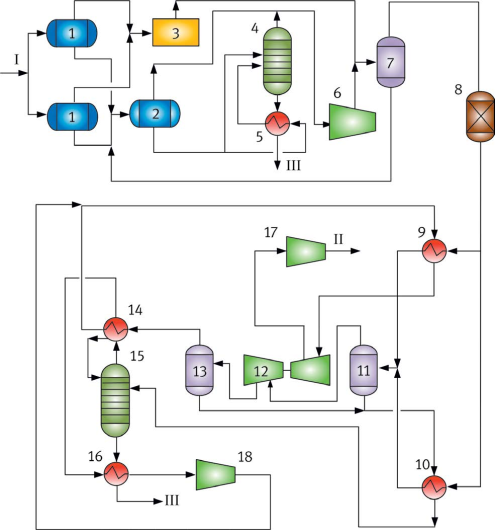
\includegraphics[width=0.45\textwidth]{assets/305}
	\caption*{Рис. 1 - Технологическая схема установки комплексной подготовки
природного газа с глубоким извлечением углеводородов
С\textsubscript{3+}}
\end{figure}

{\small I -- нестабильный газовый конденсат; II -- товарный осушенный газ; III -- деэтанизированный газовый конденсат в блок насосной внешнего транспорта
𝑀\textsubscript{сырье}=𝑀\textsubscript{газ}+𝑀\textsubscript{СНГ}+𝑀\textsubscript{СУГ}+𝑀\textsubscript{конденсат}+𝑀\textsubscript{потери}

где \emph{M}\textsubscript{сырье} - масса исходного сырья,
𝑀\textsubscript{газ} - масса товарного газа, 𝑀\textsubscript{СНГ}- масса
сжиженного нефтяного газа, \emph{M}\textsubscript{СУГ}- масса сжиженного
углеводородного газа, \emph{M}\textsubscript{конденсат} - масса
конденсата, \emph{M}\textsubscript{потери}- масса потерь.

Расчет количества товарного газа:

𝑀\textsubscript{газ}=𝑀\textsubscript{сырье}·𝐾\textsubscript{газ}

\hspace{0pt}где \emph{K}\textsubscript{газ} - коэффициент извлечения
товарного газа.

Расчет количества сжиженного нефтяного газа:

𝑀\textsubscript{СНГ}=𝑀\textsubscript{сырье}·𝐾\textsubscript{СНГ}

\hspace{0pt}где 𝐾\textsubscript{СНГ} - коэффициент извлечения сжиженного
нефтяного газа.

Расчет количества сжиженного углеводородного газа:

𝑀\textsubscript{СУГ}=𝑀\textsubscript{сырье}·𝐾\textsubscript{СУГ}

\hspace{0pt}где 𝐾\textsubscript{СУГ}- коэффициент извлечения сжиженного
углеводородного газа.

Расчет количества конденсата:

M\textsubscript{конденсат}
=M\textsubscript{сырье}·K\textsubscript{конденсат}

где 𝐾\textsubscript{конденсат}- коэффициент извлечения конденсата.

Пример расчета

Исходные данные:

Состав сырья: метан (70\%), этан (10\%), пропан (8\%), бутан (5\%),
пентан и тяжелее (7\%). Объем сырья: 10000 м³. Коэффициенты извлечения:
товарный газ (85\%), СНГ (5\%), СУГ (7\%), конденсат (3\%).

Расчет:

Масса товарного газа:

𝑀\textsubscript{газ}=10000м\textsuperscript{3}·0.85=8500м\textsuperscript{3}

Масса сжиженного нефтяного газа:

𝑀\textsubscript{СНГ}=10000м\textsuperscript{3}·0.05=500м\textsuperscript{3}

Масса сжиженного углеводородного газа:

M\textsubscript{СУГ} =10000м\textsuperscript{3}
·0.07=700м\textsuperscript{3}

Масса конденсата:

M\textsubscript{конденсат}=10000м\textsuperscript{3}·0.03=300м\textsuperscript{3}}

Таким образом, из 10000 м³ исходного сырья получается 8500 м³ товарного
газа, 500 м³ сжиженного нефтяного газа, 700 м³ сжиженного
углеводородного газа и 300 м³ конденсата.

{\bfseries Результаты и обсуждение.} Этот метод позволяет точно рассчитать
количество получаемых продуктов на основе исходных данных и
коэффициентов извлечения, что важно для планирования и оптимизации
процессов переработки углеводородного сырья. Расчет общего объема смеси
углеводородного сырья \emph{V\textsubscript{СУС}},
тыс.~м\textsuperscript{3}, определяется по следующей формуле:

\begin{equation}
V_{\text{СУС}} = V_{1} + V_{2} + V_{3} + \ldots + V_{n}
\end{equation}

где V\textsubscript{1}, V\textsubscript{2}, V\textsubscript{3}, \ldots,
V\textsubscript{n} -- объемы потоков углеводородного сырья, поступающих
в общую смесь углеводородного сырья, тыс. м\textsuperscript{3}.

Расчет доли i-того потока углеводородного сырья ꞷi, от общего количества
смеси углеводородного сырья определяется, по следующей формуле:

\begin{equation}
\omega_{i} = \frac{V_{i}}{V_{\text{СУС}}}
\end{equation}

Расчет мольной доли \emph{j}-того компонента смеси углеводородного
сырья, \emph{x\textsubscript{j}}, \%~(моль), определяется по следующей
формуле:

\begin{equation}
x_{j} = \sum_{i = 1}^{n}{x_{i}^{j} \times \omega_{i}}
\end{equation}

где, \(x_{i}^{j}\) -- мольная доля \emph{j}-того компонента,
\emph{i}-того потока углеводородного сырья поступающего в общую смесь
углеводородного сырья, \% (моль). Метод пересчета смеси углеводородного
сырья по составу и определение количества выхода продукции --
\({\ n}_{СУС}^{тг},{\ n}_{СУС}^{СУГ},{\ n}_{СУС}^{конд}\), определяется
по соотношению
\end{multicols}

\begin{equation}
\left( n_{\text{СУС}}^{\text{тг}},\ n_{\text{СУС}}^{\text{СУГ}},\ n_{\text{СУС}}^{\text{конд}},\ n_{\text{С2}}^{\text{СУС}},n_{\text{С4}}^{\text{СУС}},n_{\text{С5}}^{\text{СУС}},n_{\text{С6}}^{\text{СУС}},\ldots,n_{\text{СО2}}^{\text{СУС}},n_{N2}^{\text{СУС}},\ldots\  \right)\  = \overrightarrow{\Omega_{0}}{\times A}^{- 1}
\end{equation}

\begin{multicols}{2}
где, А -- является матрицей от состава \(\overrightarrow{\Omega_{\text{пг}}}\),
\(\overrightarrow{\Omega_{\text{суг}}}\), \(\overrightarrow{\Omega_{\text{конд}}}\):

\begin{equation}
A = \left\| \begin{array}{r}
\begin{array}{r}
\begin{array}{r}
\begin{array}{r}
\overrightarrow{\Omega_{пг}} \\
\overrightarrow{\Omega_{суг}}
\end{array} \\
\overrightarrow{\Omega_{конд}} \\
0\ 1\ 0\ 0\ 0\ 0\ 0\ 0\ 0\ 0\ldots 0 \\
0\ 0\ 0\ 1\ 0\ 0\ 0\ 0\ 0\ 0\ldots 0 \\
0\ 0\ 0\ 0\ 0\ 1\ 0\ 0\ 0\ 0\ldots 0 \\
0\ 0\ 0\ 0\ 0\ 0\ 1\ 0\ 0\ 0\ldots 0 \\
0\ 0\ 0\ 0\ 0\ 0\ 0\ 1\ 0\ 0\ldots 0 \\
0\ 0\ 0\ 0\ 0\ 0\ 0\ 0\ 1\ 0\ldots 0
\end{array} \\
0\ 0\ 0\ 0\ 0\ 0\ 0\ 0\ 0\ 1\ldots 0 \\
\ldots
\end{array} \\
0\ 0\ 0\ 0\ 0\ 0\ 0\ 0\ 0\ 0\ldots 1
\end{array} \right\|
\end{equation}

Разница между количеством углеводородного вещества в установках и
технологических трубопроводах в начале и в конце расчетного
периода,\(\ \mathrm{\Delta}\overrightarrow{Ν_{\text{запас}}}\), определяется
как:

\begin{equation}
\mathrm{\Delta}\overrightarrow{Ν_{\text{запас}}} = \left( 0,0,0,n_{\text{С2}}^{\text{СУС}},n_{\text{С4}}^{\text{СУС}},n_{\text{С5}}^{\text{СУС}},n_{\text{С6}}^{\text{СУС}},\ldots,n_{\text{СО2}}^{\text{СУС}},n_{N2}^{\text{СУС}},\ldots \right)
\end{equation}

Выражение А\textsuperscript{-1} является обозначением обратной матрицы,
определяется на основе автоматизированных методов или в соответствии
{[}11{]} осуществляется по формуле:

\begin{equation}
A^{- 1} = \frac{1}{|A|} \times S^{T}
\end{equation}

Где \(|A|\) -- определитель матрицы \emph{A};

\emph{S\textsuperscript{T}} -- транспонированная матрица
(\textbar{}\emph{A\textsubscript{ij}}\textbar)\textsubscript{~i=1\ldots n,
j=1\ldots n};

\emph{A\textsubscript{ij}} -- Алгебраическое дополнение к элементу
матрицы \emph{A} с координатами \emph{(i; j)}, определяемая по схеме:

\begin{itemize}
\item
  вычёркиваем из исходной матрицы \emph{A} i-строчку и j-й столбец.
\item
  получим новую квадратную матрицу, и её умножаем этот на
  (-1)\textsuperscript{i+j}.
\end{itemize}

Определитель матрицы рассчитывается по {[}12{]}.

Расчет (норматива) удельного количества продуктов переработки по
формулам:

\begin{equation}
k_{\text{тг}}\  = \ \frac{n_{\text{тг}}}{n_{\text{СУС}}^{\text{тг}}} + \frac{n_{\text{тг}} \times \left| \mathrm{\Delta}\overrightarrow{Ν_{\text{запас}}} \right|}{n_{\text{СУС}}}
\end{equation}

\begin{equation}
k_{\text{суг}}\  = \ \frac{n_{\text{СУГ}}}{n_{\text{СУС}}^{\text{СУГ}}} + \frac{n_{\text{СУГ}} \times \left| \mathrm{\Delta}\overrightarrow{Ν_{\text{запас}}} \right|}{n_{\text{СУС}}}
\end{equation}

\begin{equation}
k_{\text{конд}}\  = \ \frac{n_{\text{конд}}}{n_{\text{СУС}}^{\text{конд}}} + \frac{n_{\text{конд}} \times \left| \mathrm{\Delta}\overrightarrow{Ν_{\text{запас}}} \right|}{n_{\text{СУС}}}
\end{equation}

где \(n_{\text{СУС}}\) -- общее количество вещества
углеводородного сырья, поступающего на переработку, кмоль;

\(n_{\text{СУС}}^{\text{тг}}\) -- количество вещества переработанного товарного газа,
кмоль, рассчитанный на основе состава углеводородного сырья и товарного
газа в соответствии с п. 2;

\(n_{\text{СУС}}^{\text{СУГ}}\) -- количество вещества, переработанного сжиженного
углеводородного газа, кмоль, рассчитанный на основе состава
углеводородного сырья и сжиженного углеводородного газа в соответствии с
п. 2;

\(n_{\text{СУС}}^{\text{конд}}\) -- количество вещества переработанного конденсата,
кмоль, рассчитанный на основе состава углеводородного сырья и конденсата
в соответствии с п. 2;

\(n_{\text{тг}}\) - количество вещества переработанного
товарного газа, кмоль;

\(n_{\text{СУГ}}\) -- количество вещества, переработанного
сжиженного углеводородного газа, кмоль;

\emph{n}\textsubscript{конд} -- количество вещества вырабатываемого
конденсата, кмоль;

\(\mathrm{\Delta}\overrightarrow{Ν_{\text{запас}}}\) -- разница между
количеством углеводородного вещества в установках и технологических
трубопроводах в начале и в конце расчетного периода, определяемый в
соответствии п. 2.

Для определения количества выхода углеводородной продукции, входящего в
состав смеси углеводородного сырья, поступающий на переработку,
применяется следующая формула:

\begin{equation}
V_{\text{тг}}^{\text{вых}}\  = 24,04012 \times n_{\text{тг}}{\times k}_{\text{тг}},\text{ ст.м}^3
\end{equation}

\begin{equation}
m_{\text{СУГ}}^{\text{вых}}\  = n_{\text{СУГ}}{\times k}_{\text{СУГ}} \times M_{\text{СУГ}}, \text{кг}
\end{equation}

\begin{equation}
m_{\text{конд}}^{\text{вых}}\  = n_{\text{конд}}{\times k}_{\text{конд}} \times M_{\text{конд}}, \text{кг}
\end{equation}

где \emph{n\textsubscript{ТГ}} -- количество вещества переработанного
товарного газа, кмоль, рассчитанный на основе состава смеси
углеводородного сырья и товарного газа в соответствии с Разделом 3;

\emph{n\textsubscript{СУГ}} -- количество вещества, переработанного
сжиженного углеводородного газа, кмоль, рассчитанный на основе состава
смеси углеводородного сырья и сжиженного углеводородного газа в
соответствии с Разделом 3;

\emph{n\textsubscript{конд}} -- количество вещества переработанного
конденсата, кмоль, рассчитанный на основе состава смеси углеводородного
сырья и конденсата в соответствии с Разделом~3;

\emph{k}\textsubscript{тг} \emph{--} удельная норма выхода
переработанного товарного газа;

\emph{k}\textsubscript{СУГ} \emph{--} удельная норма выхода
переработанного сжиженного углеводородного газа;

\emph{k}\textsubscript{конд} \emph{--} удельная норма выхода
переработанного конденсата;

\emph{М}\textsubscript{СУГ} \emph{--} мольная масса переработанного
сжиженного углеводородного газа, кг/кмоль;

\emph{М}\textsubscript{конд} \emph{--} мольная масса переработанного
конденсата, кг/кмоль.

{\bfseries Контроль точности расчета}

Расширенная неопределённость результатов расчета выхода углеводородного
сырья, тыс.~м\textsuperscript{3}, определяется по формуле:

\begin{equation}
U = k \cdot u_{l}
\end{equation}

где \emph{l} -- коэффициент охвата, принимает значение в интервале 2-3,
что соответствует выбранному уровню доверия 95-99 \%;

\emph{u\textsubscript{k}} -- стандартная неопределённость,
тыс.~м\textsuperscript{3}, определяемая по формуле:

\begin{equation}
u_{k} = \sum_{i = 0}^{n}{V_{i} \cdot \mathrm{\Delta}\Omega_{i}} + \sum_{j = 0}^{m}{V_{j} \cdot \delta_{j}}
\end{equation}

где \emph{V} -- общий объем смеси углеводородного сырья, поступающий на
переработку, в расчетный период, тыс.~м\textsuperscript{3};

\emph{ΔΩ\textsubscript{i}} -- установленная погрешность определения
компонентного состава\\
\emph{i}-го анализа;

\emph{V\textsubscript{i}} -- количество газа, соответствующего
компонентному составу полученному \emph{i}-ым анализом, в расчетный
период, тыс.~м\textsuperscript{3}, участвующим в учете газа в системе
переработки углеводородного сырья;

\emph{δ\textsubscript{j}} -- установленная погрешность \emph{j}-го
замерного узла, в соответствии с таблицей Е.1;

\emph{V\textsubscript{j}} -- количество зафиксированного газа
\emph{j}-ым замерным узлом, в расчетный период,
тыс.~м\textsuperscript{3}, участвующим в учете газа в системе
переработки углеводородного сырья.

Контроль правильности результатов расчета:

\begin{equation}
\frac{u_{l}}{V} \times 100 < K_{n}
\end{equation}

где \emph{V} -- общий объем смеси углеводородного сырья, поступающий на
переработку, в расчетный период, тыс.~м\textsuperscript{3};

\emph{u\textsubscript{l}} -- стандартная неопределённость, определяемая
по формуле (15), тыс.~м\textsuperscript{3};

\emph{K\textsubscript{n}} -- норматив контроля, \%;

\emph{K\textsubscript{n}} принимается не более 1\%.

Для перевода количества вещества в массу смеси углеводородного сырья
применяется следующая формула:

\begin{equation}
m_{\text{СУС}}\  = n \times M_{\text{УС}}, \text{кг},
\end{equation}

где \emph{n}~--~количество вещества смеси углеводородного сырья, кмоль;

\emph{M\textsubscript{УС}}~--~молярная масса смеси углеводородного
сырья, кг/кмоль.

Для перевода массу в количество вещества смеси углеводородного сырья
применяется следующая формула:

\begin{equation*}
n = \frac{m_{\text{УС}}}{M_{\text{УС}}}, \text{кмоль},
\end{equation*}

где, \emph{m\textsubscript{УС}}~--~масса смеси углеводородного сырья,
кг;

\emph{M\textsubscript{УС}}~--~молярная масса смеси углеводородного
сырья, кг/кмоль.

Для перевода количества вещества в объем газа в стандартных условиях
смеси углеводородного сырья применяется следующая формула:

\begin{equation}
V_{\text{ст.у.}} = 24,04012 \times n, \text{м}^3
\end{equation}

где \emph{n} --~количество вещества смеси углеводородного сырья, кмоль.

Для перевода объем газа (в стандартных условиях) в количество вещества
смеси углеводородного сырья применяется следующая формула:

\begin{equation}
n = 0,04159713 \times V_{\text{ст.у.}}, \text{кмоль}
\end{equation}

Где \emph{V\textsubscript{ст.у.}}~--~объем углеводородного газа в
стандартных условиях, м\textsuperscript{3}.

Молярные массы компонентов смеси углеводородного сырья приведены в
таблице А.1.

Плотность газа в стандартных условиях, \emph{ρ},
кг/м\textsuperscript{3}, определяется по формуле:

ρ = 0,04159713⋅М (20)

где \emph{М} -- молярная масса, кг/кмоль.

Экологические и экономические аспекты. Научно-исследовательская работа
по разработке и анализу методов переработки углеводородного сырья
предлагает инновационные решения, которые существенно повышают
экономическую эффективность и снижают экологическую нагрузку.
Использование передовых технологий и точных аналитических методов
позволяет улучшить переработку сырья, снизить затраты и повысить доходы,
одновременно способствуя охране окружающей среды за счет снижения
выбросов и рационального использования ресурсов. Точные методы расчета и
оптимизация технологических процессов позволяют уменьшить объемы
сжигания газа на факелах, что снижает выбросы загрязняющих веществ и
парниковых газов в атмосферу. Внедрение современных технологий
переработки углеводородного сырья способствует снижению экологической
нагрузки и улучшению экологических показателей предприятий. Оптимизация
переработки углеводородного сырья позволяет рационально использовать
ресурсы, минимизируя потери и воздействие на окружающую среду.
Применение энергоэффективных технологий, таких как мембранные,
адсорбционные и абсорбционные процессы, улучшает процессы переработки и
снижает энергозатраты, что благоприятно сказывается на экологии.
Современные методы переработки, такие как низкотемпературная
ректификация и использование высокоэффективных насадок в колоннах,
уменьшают энергозатраты и выбросы, повышая экологическую безопасность
процессов. Методы расчета материального баланса и аналитические
технологии позволяют точно определять количество выходящих продуктов
(товарный газ, сжиженный углеводородный газ, конденсат), что улучшает
планирование и управление ресурсами, повышая рентабельность
производственных процессов. Оптимизация технологических процессов и
использование передовых математических методов позволяют достичь высокой
точности и надежности расчетов, что улучшает планирование и управление
ресурсами. Применение передовых технологий, таких как плазмохимические и
волновые методы, снижает капитальные затраты на переработку
углеводородного сырья, улучшая экономические показатели предприятий.
Разработка методов переработки газа непосредственно на месте его добычи
снижает затраты на транспортировку, что особенно важно для удаленных
месторождений. Внедрение автоматизированных систем расчетов сокращает
время на проведение расчетов и снижает вероятность ошибок, что
дополнительно повышает экономическую эффективность переработки
углеводородного сырья. Продажа единиц сокращения выбросов (ЕСВ) помогает
улучшить экономические показатели проектов и компенсировать часть затрат
на создание инфраструктуры для утилизации попутного нефтяного газа
(ПНГ).

{\bfseries Выводы:} Уникальный разработанный метод предлагает расчет общего
объема смеси углеводородного сырья, а также доли каждого потока сырья в
общей смеси. Это позволяет точно определить мольную долю каждого
компонента в смеси. Применение матричных методов для пересчета состава
углеводородного сырья на выход продукции. Использование обратной матрицы
и компонентного состава позволяет точно определить количество выходящих
продуктов. Методика включает расчет удельного выхода различных продуктов
(товарный газ, сжиженный углеводородный газ, конденсат) на основе общего
количества углеводородного сырья и технологических потерь. Определение
количества выходящей продукции для каждого конкретного потока
углеводородного сырья позволяет детализировать расчет и повысить
точность. Введение показателя расширенной неопределенности и методов
контроля правильности расчетов. Это обеспечивает уверенность в точности
и достоверности результатов. Применение формул для перевода количества
вещества в массу и объем и наоборот. Это позволяет легко конвертировать
результаты расчетов в необходимые единицы измерения.
\end{multicols}

\begin{center}
{\bfseries Литература}
\end{center}

\begin{noparindent}
1.Муллахметова Л.И., Черкасова Е.И. Попутный нефтяной газ: подготовка,
транспортировка и переработка// Вестник Казанского технологического
университета.- 2015. - Т.18(19)- С. 83-90

2.Азарова А.И. Инновационные технологии в нефтедобыче и их отражение в
системе управления вертикально интегрированных нефтяных компаний//
Проблемы учёта и финансов.-2012.- № 4 (8) 2012. С.35-47

3.Владимиров А.И. Экология нефтегазового комплекса /А.И. Владимиров. М:
Нефть и газ.- 2003.- 415 с. ISBN 5-7246-0232

4.Муллахметова Л.И., Черкасова Е.И., Сигбатуллина Р.И., Бикмухаметова
Г.К., Мустафина А.М., Салахов И.И. Газофракционирование // Вестник
технологического университета.- 2016.- Т19(24) - С. 49-555.

5.Семенова Т.А. Очистка технологических газов / Т.А. Семенова и др -M.:
Химия- 1997.-314 с.

6.Абдуллин А.И., Солодова Н.Л., Пиролиз углеводородного сырья. Учебное
пособие / Солодова Н.Л., Абдуллин А.И.// КГТУ. - Казань, 2008.- 240 с.
ISBN:~978-5-7882-0518-2

7.Аджиев А.Ю., Пуртов П.А. Подготовка и переработка попутного нефтяного
газа в России: в 2 ч. Ч. 2 / А.Ю.Аджиев, П.А.Пуртов. - Краснодар: ЭДВИ,
2014. - 504 с.

8.Ибрагимова А.В. Методическое обеспечение управления эффективностью
утилизации попутного нефтяного газа на нефтедобывающих предприятиях:
дис. \ldots{} к.э.н. Удмуртский государственный университет. -2015. --
166 с.

9.Муродов М. Н. Системы разработки газоконденсатных месторождений //
Молодой ученый.- 2014.- №1.- С. 102-103.

10.Аристова В.В. Альтернативные комплексные технологии переработки
попутных нефтяных газов/ В.В. Аристова, А.С. Дорофеев
(http://www.gazcompany.ru/gazpngfull.html)

11.Даутов Р.З., Тимербаев М.Р. Численные методы. Решение задач линейной
алгебры и дифференциальных уравнений: учебное пособие. --- Казань:
К(П)ФУ, 2021.-168 с.

12.Кабанова О.А. Вычисление определителя. Нахождение обратной матрицы/
Мет. пособие по курсу «Высшая математика» раздел «Линейная алгебра». М.:
МАИ, 2015. -- 15 с.
\end{noparindent}

\begin{center}
{\bfseries References}
\end{center}

\begin{noparindent}
1.Mullahmetova L.I., Cherkasova E.I. Poputnyj neftjanoj gaz: podgotovka,
transportirovka i pererabotka// Vestnik Kazanskogo tehnologicheskogo
universiteta.- 2015. - T.18(19)- S. 83-90.

{[}in Russ.{]}

2.Azarova A.I. Innovacionnye tehnologii v neftedobyche i ih otrazhenie v
sisteme upravlenija vertikal\textquotesingle no integrirovannyh
neftjanyh kompanij// Problemy uchjota i finansov.-2012.- № 4 (8) 2012.
S.35-47. {[}in Russ.{]}

3.Vladimirov A.I. Jekologija neftegazovogo kompleksa /A.I. Vladimirov.
M: Neft\textquotesingle{} i gaz.- 2003.- 415 s. ISBN 5-7246-0232. {[}in
Russ.{]}

4.Mullahmetova L.I., Cherkasova E.I., Sigbatullina R.I., Bikmuhametova
G.K., Mustafina A.M., Salahov I.I. Gazofrakcionirovanie // Vestnik
tehnologicheskogo universiteta.- 2016.- T19(24) - S. 49-555. {[}in
Russ.{]}

5.Semenova T.A. Ochistka tehnologicheskih gazov / T.A. Semenova i dr
-M.: Himija- 1997.-314 s.

6.Abdullin A.I., Solodova N.L., Piroliz uglevodorodnogo
syr\textquotesingle ja. Uchebnoe posobie / Solodova N.L., Abdullin
A.I.// KGTU. - Kazan\textquotesingle, 2008.- 240 s. ISBN:
978-5-7882-0518-2. {[}in Russ.{]}

7.Adzhiev A.Ju., Purtov P.A. Podgotovka i pererabotka poputnogo
neftjanogo gaza v Rossii: v 2 ch. Ch. 2 / A.Ju.Adzhiev, P.A.Purtov. -
Krasnodar: JeDVI, 2014. - 504 s. {[}in Russ.{]}

8.Ibragimova A.V. Metodicheskoe obespechenie upravlenija
jeffektivnost\textquotesingle ju utilizacii poputnogo neftjanogo gaza na
neftedobyvajushhih predprijatijah: dis. \ldots{} k.je.n. Udmurtskij
gosudarstvennyj universitet. -2015. -- 166 s. {[}in Russ.{]}

9.Murodov M. N. Sistemy razrabotki gazokondensatnyh mestorozhdenij //
Molodoj uchenyj.- 2014.- № 1.- S. 102-103. {[}in Russ.{]}

10.Aristova V.V. Al\textquotesingle ternativnye kompleksnye tehnologii
pererabotki poputnyh neftjanyh gazov/ V.V. Aristova, A.S. Dorofeev
(http://www.gazcompany.ru/gazpngfull.html). {[}in Russ.{]}

11.Dautov R.Z., Timerbaev M.R. Chislennye metody. Reshenie zadach
linejnoj algebry i differencial\textquotesingle nyh uravnenij: uchebnoe
posobie. --- Kazan\textquotesingle: K(P)FU, 2021.-168 s. {[}in Russ.{]}

12.Kabanova O.A. Vychislenie opredelitelja. Nahozhdenie obratnoj
matricy/ Met. posobie po kursu «Vysshaja matematika» razdel «Linejnaja
algebra». M.: MAI, 2015.- 15 s. {[}in Russ.{]}
\end{noparindent}

\emph{{\bfseries Сведения об авторах}}

\begin{noparindent}
Сейлханов К.К. - магистр математики, директор Товарищество с
ограниченной ответственностью «ГЦПК «Кəсіпкер», Астана, Казахстан,
e-mail: kks\_kz@mail.ru;Мурзагалиев Б.Т. - магистр по специальности
«Химическая технология взрывчатых веществ и пиротехнических средств»,
технический Директор Товарищество с ограниченной ответственностью

«ГЦПК «Кəсіпкер, Астана, Казахстан, e-mail:
murzagaliyev.b.t@gmail.com;Даулетжанова Ж.Т. - доктор PhD,
преподаватель, Казахский университет технологии и бизнеса им.
К.Кулажанова, Астана, Казахстан, e-mail: kaliyeva\_zhanna@mail.ru;

Сейлханова М.Т. - магистр педагогических наук, научный сотрудник
Товарищество с ограниченной ответственностью «ГЦПК «Кəсіпкер», Астана,
Казахстан, e-mail: mbt\_kz@mail.ru;

Бахтияр С. - магистр педагогических наук начальник отдела
Нормативно-технической документации Товарищество с ограниченной
ответственностью «ГЦПК «Кəсіпкер»,Астана, Казахстан, e-mail:
serik19.98.01@gmail.com
\end{noparindent}

\emph{{\bfseries Information about authors}}

\begin{noparindent}
Seilkhanov K.K.- Director of Limited liability partnership «ГЦПК
«Кəсіпкер», Astana, Kazakhstan, Master of Mathematics, e-mail:
kks\_kz@mail.ru;

Murzagaliev B.T. - Technical Director of Limited liability partnership
«ГЦПК «Кəсіпкер», Astana, Kazakhstan, Master\textquotesingle s degree in
"Chemical technology of explosives and pyrotechnics", e-mail:
murzagaliyev.b.t@gmail.com;

Dauletzhanova Zh.T. - PhD, Lecturer, Kazakh University of Technology and
Business, Astana, Kazakhstan, e-mail: kaliyeva\_zhanna@mail.ru;

Seilkhanova M.T. - Researcher of Limited liability partnership «ГЦПК
«Кəсіпкер»,Astana, Kazakhstan, Master of Educational Sciences, e-mail:
mbt\_kz@mail.ru;

Bakhtiyar S. - Head of the Regulatory and Technical Documentation
Department in Limited liability partnership «ГЦПК «Кəсіпкер», Astana,
Kazakhstan, Master of Educational Sciences, e-mail:
serik19.98.01@gmail.com
\end{noparindent}
